\documentclass[letterpaper, 10 pt, conference]{ieeeconf}  % Comment this line out if you need a4paper

%\documentclass[a4paper, 10pt, conference]{ieeeconf}      % Use this line for a4 paper

\IEEEoverridecommandlockouts                              % This command is only needed if 
                                                          % you want to use the \thanks command

\overrideIEEEmargins                                      % Needed to meet printer requirements.

%In case you encounter the following error:
%Error 1010 The PDF file may be corrupt (unable to open PDF file) OR
%Error 1000 An error occurred while parsing a contents stream. Unable to analyze the PDF file.
%This is a known problem with pdfLaTeX conversion filter. The file cannot be opened with acrobat reader
%Please use one of the alternatives below to circumvent this error by uncommenting one or the other
%\pdfobjcompresslevel=0
%\pdfminorversion=4

% See the \addtolength command later in the file to balance the column lengths
% on the last page of the document

% The following packages can be found on http:\\www.ctan.org
\usepackage{graphics} % for pdf, bitmapped graphics files
\usepackage{epsfig} % for postscript graphics files
\usepackage{mathptmx} % assumes new font selection scheme installed
\usepackage{times} % assumes new font selection scheme installed
\usepackage{amsmath} % assumes amsmath package installed
\usepackage{amssymb}  % assumes amsmath package installed

\title{\LARGE \bf
Preparation of Papers for IEEE Sponsored Conferences \& Symposia
}

\author{Albert Author$^{1}$ and Bernard D. Researcher$^{2}$}

\begin{document}

\maketitle
\thispagestyle{empty}
\pagestyle{empty}


%%%%%%%%%%%%%%%%%%%%%%%%%%%%%%%%%%%%%%%%%%%%%%%%%%%%%%%%%%%%%%%%%%%%%%%%%%%%%%%%
\begin{abstract}

This electronic document is a live template. 

\end{abstract}

%%%%%%%%%%%%%%%%%%%%%%%%%%%%%%%%%%%%%%%%%%%%%%%%%%%%%%%%%%%%%%%%%%%%%%%%%%%%%%%%
\section{INTRODUCTION}

This template provides authors with most of the formatting specifications needed for preparing electronic versions of their papers. 

\section{PROCEDURE}

\subsection{Simulation Environment}
The simulation environment was set as a 500 by 500 pixel virtual space, where the simulation agents could move in two dimensions. (Figure \ref{fig:sim_env}). The size of each agent was defiend as the radius of 5 pixel circle. Therefore, when more than two agents approached each other at the distance of closer than 5 pixel, those agents' collision count was added. In one trial, all agents moved 500 steps.

\subsection{Avoidance Algorithms}
Based on the collision avoidance algorithms, agents were classified into two types.

For one of types, simple avoidance agent, their avoindace vectors were generated to the opposite direction of the other agents which approached within a 50 pixel. The size of avoidance vectors were fixed as either 1, 2, 3, 4, or 5 pixel in one trial. 
For another type of agent, which we call as the dynamic avoidance agent, their avoidance vector were generated based on the braking index. When an agent approch to another agent within 50 pixel, the braking rate was calculated based on their relative positions and speeds, and their avoidance vectors were determined from 1 to 3 pixel. This way of avoidance enabled agents to avoid other agents considering how much potential danger they are facing; in safer situations, agents avoid slightly, on the contrary, in more dangerous situation, agents avoid widely not to collide each other. 

\begin{figure}[thpb]
   \centering
   \framebox{\parbox{3in}{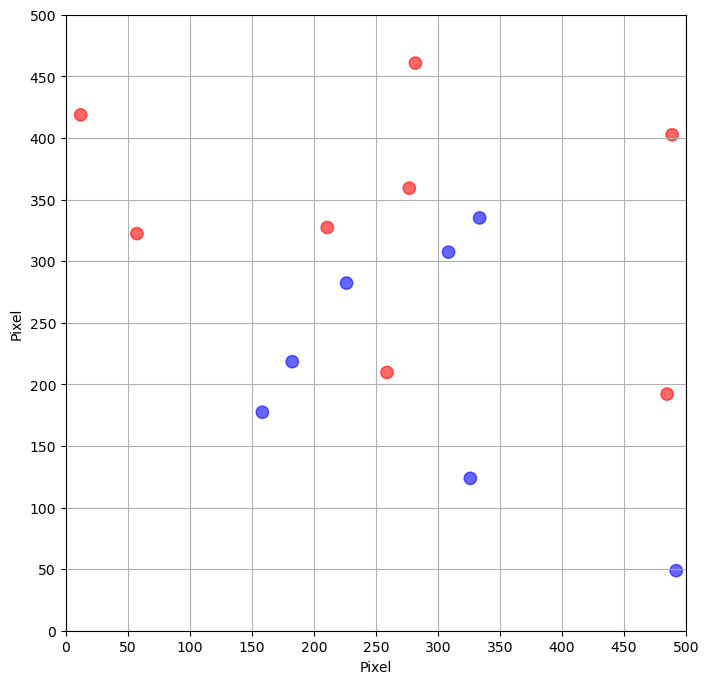
\includegraphics[scale=0.3]{fig1.png}}}
   \caption{Overview of the simulation environment}
   \label{fig:sim_env}
\end{figure}

\section{MATH}

Before you begin to format your paper, first write and save the content as a separate text file. 

\subsection{Abbreviations and Acronyms} Define abbreviations and acronyms the first time they are used in the text, even after they have been defined in the abstract. 

\subsection{Units}

\begin{itemize}

\item Use either SI (MKS) or CGS as primary units. 

\end{itemize}


\subsection{Equations}

The equations are an exception to the prescribed specifications of this template. 

$$z
\alpha + \beta = \chi \eqno{(1)}
$$

Note that the equation is centered using a center tab stop. 

\subsection{Some Common Mistakes}
\begin{itemize}


\item The word data is plural, not singular.

\end{itemize}


\section{USING THE TEMPLATE}

Use this sample document as your LaTeX source file to create your document. 

\subsection{Headings, etc}

Text heads organize the topics on a relational, hierarchical basis. 

\subsection{Figures and Tables}

Positioning Figures and Tables.

\begin{table}[h]
\caption{An Example of a Table}
\label{table_example}
\begin{center}
\begin{tabular}{|c||c|}
\hline
One & Two\\
\hline
Three & Four\\
\hline
\end{tabular}
\end{center}
\end{table}


   \begin{figure}[thpb]
      \centering
      \framebox{\parbox{3in}{We suggest that you use a text box to insert a graphic because, in an document, this method is somewhat more stable than directly inserting a picture.}}

      %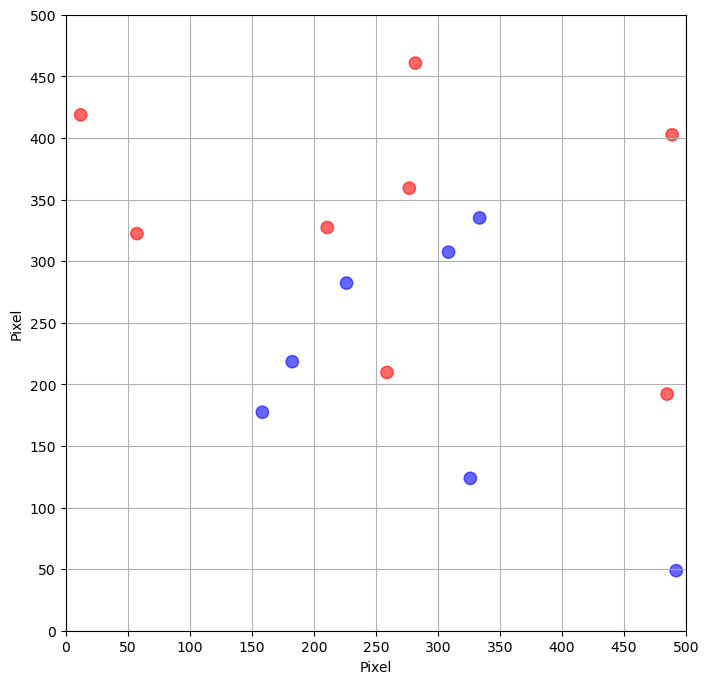
\includegraphics[scale=0.3]{fig1.png}
      \caption{Inductance of oscillation winding on amorphous
       magnetic core versus DC bias magnetic field}
      \label{figurelabel}
   \end{figure}
   

Figure Labels: Use 8 point Times New Roman for Figure labels. 

\section{CONCLUSIONS}

A conclusion section is not required. Although a conclusion may review the main points of the paper, do not replicate the abstract as the conclusion. A conclusion might elaborate on the importance of the work or suggest applications and extensions. 

\addtolength{\textheight}{-12cm}  

\section*{APPENDIX}

Appendixes should appear before the acknowledgment.

\section*{ACKNOWLEDGMENT}

The preferred spelling of the word on the first page.


\begin{thebibliography}{99}

\bibitem{c1} G. O. Young, Synthetic structure of industrial plastics (Book style with paper title and editor), in Plastics, 2nd ed. vol. 3, J. Peters, Ed.  New York: McGraw-Hill, 1964, pp. 1564.

\end{thebibliography}




\end{document}
